\documentclass{article}
\usepackage{nips07submit_e,times}

\usepackage{url}

\usepackage[plain]{algorithm}
\usepackage{algpseudocode}

\usepackage{graphicx}
\usepackage{subfigure} 

\usepackage{bm}

\usepackage{booktabs}

\usepackage[tbtags]{amsmath}
\usepackage{amssymb,rotating,multirow}

\usepackage{color}
\newcommand{\note}[1]{\textcolor{red}{[#1]}}

\newcommand{\comment}[1]{}

% just to help while drafting the paper
\usepackage{color}
\newcommand{\todo}{\textcolor{red}}

\def\balpha{\pmb{\alpha}}
\def\bbeta{\pmb{\beta}}
\def\bgamma{\pmb{\gamma}}
\def\blambda{\pmb{\lambda}}
\def\bmu{\pmb{\mu}}
\def\bnu{\pmb{\nu}}
\def\bomega{\pmb{\omega}}
\def\bphi{\pmb{\phi}}
\def\bpi{\pmb{\pi}}
\def\bTheta{\pmb{\Theta}}

\def\ba{\pmb{a}}   
\def\bb{\pmb{b}}   
\def\bc{\pmb{c}}   
\def\bbf{\pmb{f}}   
\def\bg{\pmb{g}}   
\def\bm{\pmb{m}}   
\def\bn{\pmb{n}}   
\def\bp{\pmb{p}}   
\def\bq{\pmb{q}}   
\def\bu{\pmb{u}}   
\def\bw{\pmb{w}}   
\def\bx{\pmb{x}}   
\def\by{\pmb{y}}   
\def\bz{\pmb{z}}   
\def\bzero{\pmb{0}}
\def\bA{\pmb{A}}   
\def\bB{\pmb{B}}   
\def\bC{\pmb{C}}   
\def\bI{\pmb{I}}   
\def\bN{\pmb{N}}   
\def\bQ{\pmb{Q}}   
\def\bX{\pmb{X}}   
\def\bZ{\pmb{Z}}   
\def\bS{\pmb{S}}   

\def\g{\,|\,}   

\newcommand{\is}{:=}

\newtheorem{thm}{Theorem}[section]
\newtheorem{cor}[thm]{Corollary}
\newtheorem{conj}[thm]{Conjecture}


\title{Supplementary Materials for \\ ``An Alternative Prior Process for\\
Nonparametric Bayesian Clustering"}


\author{
{\bf Hanna M. Wallach}\\
Department of Computer Science \\
University of Massachusetts Amherst \\
Address \\
\texttt{wallach@cs.umass.ed} \\
\And
{\bf Shane T. Jensen}\\
Department of Statistics, The Wharton School\\
University of Pennsylvania\\
Philadelphia, PA 19104 \\
\texttt{stjensen@wharton.upenn.edu} \\
\AND
{\bf Lee Dicker} \\
Department of Biostatistics\\
Harvard School of Public Health\\
Boston, MA \\
\texttt{ldicker@hsph.harvard.edu} \\
\And
{\bf Katherine Heller} \\
Gatsby Computational Neuroscience Unit \\
University College London \\
London, UK \\
\texttt{heller@gatsby.ucl.ac.uk} \\
}

% The \author macro works with any number of authors. There are two commands
% used to separate the names and addresses of multiple authors: \And and \AND.
%
% Using \And between authors leaves it to \LaTeX{} to determine where to break
% the lines. Using \AND forces a linebreak at that point. So, if \LaTeX{}
% puts 3 of 4 authors names on the first line, and the last on the second
% line, try using \AND instead of \And before the third author name.

\newcommand{\fix}{\marginpar{FIX}}
\newcommand{\new}{\marginpar{NEW}}

\begin{document}

\makeanontitle

\section{Proof of Square Root Law for $\mathbb{E}\,(K_N\g{\rm UN})$} \label{UNmomresults}

We define $T_k = \inf\, \{ m > T_{k-1} ; X_m \notin \{X_1, \ldots, X_{m-1} \}\}$.  $T_k$ is the ``waiting time" (number of observations needed) until the $k$-th new cluster generated by the uniform process.   Under the uniform process, $T_k = \sum_{i=1}^k \tau_i$ where $\tau_i \sim {\rm Geometric}\, (\theta\,/\,(\theta + i - 1)$ and the $\tau_i$'s are independent, so 
\begin{align}
\mathbb{E}\, (T_k) &= \sum\limits_{i=1}^k \frac{\theta + i - 1}{\theta} = \frac{k^2}{2 \theta} + k \left( 1 - \frac{1}{2 \theta} \right) \label{eTk} \\
 {\rm Var}\, (T_k) &= \sum\limits_{i=1}^k \frac{(\theta + i - 1)\,(i - 1)}{\theta^2} = \frac{k^3}{3 \theta^2} + k^2 \frac{1}{2\theta} \left( 1 - \frac{1}{\theta} \right) + k \frac{1}{2\theta} \left( \frac{1}{3 \theta} - 1 \right) \hspace{1.25cm} \label{vTk}
\end{align}
In terms of $T_j$,  $K_N = \max \{ j ; T_j \leq N \} = \sum_{j=1}^N
{\rm I}\, (T_j \leq N)$.     We first prove a strong law for the
convergence of $T_k$.  Let $\epsilon > 0$.  From Chebychev's
inequality and (\ref{vTk}), we have
\begin{align}
{\rm P}\, \left(|T_k - \mathbb{E}\, (T_k) | > \epsilon  k^2\right) \leq \frac{{\rm Var}\, (T_k) }{\epsilon^2k^4}  \leq \frac{C(\theta,\epsilon)}{k} \label{Cheby}
\end{align}
From (\ref{Cheby}), we have that, 
\begin{align*}
{\rm P}\, \left(|T_{k^2} - \mathbb{E}\, (T_{k^2})| > \epsilon k^4 \right) \leq \frac{C(\theta,\epsilon)}{k^2} 
\end{align*} 
and so by the  Borel-Cantelli lemma, we have ${\rm P}\, \left(|T_{k^2} - \mathbb{E}\,(T_{k^2})| > \epsilon k^4 \right) = 0.$
Since $\epsilon > 0$ was chosen arbitrarily, it follows that $\frac{T_{k^2} - \mathbb{E}\,(T_{k^2})}{k^4} \to 0$ almost surely and hence 
$\frac{T_{k^2}}{k^4} \to \frac{1}{2\theta}$ almost surely. Now, let $m = \lfloor \sqrt{k} \rfloor$.  Since $T_k$ is
increasing, we have the following inequality:
\begin{align}
\frac{T_{m^2}}{(m + 1)^4} \leq \frac{T_k}{k^2} \leq
\frac{T_{(m + 1)^2}}{m^4}.   \label{subseq}
\end{align}
Since $\frac{m + 1}{m} \to 1$, both sides of the inequality (\ref{subseq}) converge to $(2\theta)^{-1}$ almost surely, and so 
\begin{align}
\frac{T_k}{k^2} \to \frac{1}{2\theta} \hbox{ almost surely.}  \label{strongTk}
\end{align}
The strong law (\ref{strongTk}) implies a strong law for $K_N$ as follows. $T_{K_N} \leq N < T_{K_N + 1}$ and, consequently,
\begin{align*}
\frac{T_{K_N}}{K_N^2} \leq \frac{n}{K_N^2} < \frac{T_{K_N +
1}}{K_N^2}.
\end{align*}
Since $K_N \to \infty$ almost surely and $T_k\,/\,k^2 \to 1\,/\,(2\theta)$ almost surely, it follows that the left and
right hand side above both converge to $1/(2\theta)$ almost surely.  Thus, $K_N^2 \,/\, N \to 2\theta$ almost surely and so
\begin{align}
\frac{K_N}{\sqrt{N}} \to \sqrt{2\theta} \hbox{ almost surely.}   \label{strongKn}
\end{align}
From the strong law (\ref{strongKn}) and the dominated convergence theorem, we have 
\begin{align}
\frac{\mathbb{E}\,(K_N)}{N} \to 0.  \label{Kngoingtozero}
\end{align}
We combine (\ref{Kngoingtozero}) together with following result (derived in section~\ref{momentlemma} below), 
\begin{align}
\mathbb{E}\,(K_N^2) = \mathbb{E}\,(K_N) + 2\theta\,(N - \mathbb{E}\,(K_N)). \label{twomoments}
\end{align}
to give us 
\begin{align}
\frac{\mathbb{E}\,(K_N^2)}{N} \to 2\theta. \label{Knsquaredgoingtotheta}
\end{align}
Finally, using (\ref{Knsquaredgoingtotheta}) together with Fatou's lemma and Jensen's inequality, gives us
\begin{align*}
\sqrt{2\theta} \leq \liminf_{N \to \infty} \frac{\mathbb{E}\,(K_N)}{\sqrt{N}} \leq
\limsup_{N \to \infty} \frac{\mathbb{E}\,(K_N)}{\sqrt{N}} \leq \limsup_{N \to
\infty} \sqrt{\frac{\mathbb{E}\,(K_N^2)}{N}} = \sqrt{2\theta}.
\end{align*}
which proves the result
\begin{align*}
\frac{\mathbb{E}\,(K_N)}{\sqrt{N}} \to \sqrt{2\theta}.
\end{align*}
under the uniform process. 

\section{Result relating $\mathbb{E}\,(K_N)$ to  $\mathbb{E}\,(K_N^2)$} \label{momentlemma}

Recall the definition of $T_j$ from above and now define $M_N = K_N +
1$.  Consider the ``waiting time" $T_{M_N}$ until the observation that
creates the $(K_N + 1)^{\textrm{th}}$ unique cluster.  We relate
$\mathbb{E}\,(K_N)$ to  $\mathbb{E}\,(K_N^2)$ by calculating
$\mathbb{E}\, (T_{M_N})$ in two different ways.  First, observe that
we have
\begin{align*}
\mathbb{E}\, (T_{M_N}) &= \mathbb{E}\,
\left(\sum\limits_{k=1}^\infty \tau_k \cdot {\rm I}\, (k \leq M_N)
\right) = \sum\limits_{k=1}^\infty \mathbb{E}\, (\tau_k) \cdot {\rm P}\,
(k \leq M_N) \\ &= \frac{\theta -1}{\theta}\,
\sum\limits_{k=1}^\infty {\rm P}\, (k \leq M_N) + \frac{1}{\theta}
\sum\limits_{k=1}^\infty k \cdot {\rm P}\, (k \leq M_N) \\ &=
\frac{\theta -1}{\theta}\, \mathbb{E}\, (M_N) + \frac{1}{2 \theta}\,
\mathbb{E}\, (M_N (M_N + 1))
\end{align*}
which, since $M_N = K_N + 1$, simplifies to 
\begin{align}
\mathbb{E}\, (T_{M_N})  = 1 + \mathbb{E}\, (K_N) \left( 1 + \frac{1}{2 \theta} \right) + \mathbb{E}\, (K_N^2)\, \frac{1}{2 \theta}.   \label{lemmaeq1}
\end{align}
$T_{M_N} = N + \sum_{j} {\rm I}\, (M_{N + j} = M_N)$ and so $\mathbb{E}\, (T_{M_N}) = N + \sum_{j} {\rm P}\, (M_{N + j} = M_N)$ where 
\begin{align*}
{\rm P}\,(M_{N + j} = M_N) &= \sum_k {\rm P}\,(T_k \leq N, \ N + j < T_{k + 1}) \\
&= \sum_k {\rm P}\,(T_k \leq N < T_{k + 1})\, {\rm P}\,(j < \tau_{k + 1}) \\
&= \sum_k {\rm P}\,(M_N = k + 1)\, {\rm P}\,(j < \tau_{k + 1}).
\end{align*}
It follows that
\begin{align*}
\mathbb{E}\,(T_{M_N}) &= n + \sum_j \sum_k {\rm P}\,(M_N = k + 1)\, {\rm P}\,(j < \tau_{k + 1}) \\
&= N + \sum_k {\rm P}\,(M_N = k + 1)\,  \sum_j {\rm P}\,(j < \tau_{k + 1}) \\
&= N + \sum_k {\rm P}\,(M_N = k + 1)\, \mathbb{E}\,(\tau_{k + 1}) \\
&= N + \sum_k {\rm P}\,(K_N = k)\, \frac{k+\theta}{\theta} \\
\end{align*}
which can be simplified to 
\begin{align}
\mathbb{E}\,(T_{M_N})  = N + 1 + \mathbb{E}\,(K_N)\, \frac{1}{\theta}   \label{lemmaeq2}
\end{align}
Combining (\ref{lemmaeq1}) and (\ref{lemmaeq2}) gives (\ref{twomoments}): 
\begin{align*}
\mathbb{E}\,(K_N^2) = \mathbb{E}\,(K_N) + 2\theta\,(N - \mathbb{E}\,(K_N)). 
\end{align*}

\section{Graphical Model for Document Clustering}

\begin{figure}[ht!]
\begin{center}
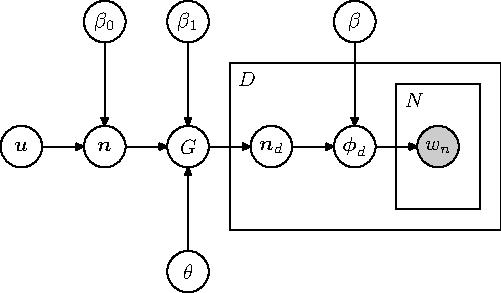
\includegraphics[scale=0.75]{figures/dpmm_fixed-1.pdf}
\end{center}
\caption{Word-based mixture model. $G$ is either drawn from a
  Dirichlet process or a uniform process. Variables $\bn$, $\bu$, $\beta_1$
  and $\beta_0$ comprise the hierarchical Dirichlet base
  measure $G_0$.}
\label{fig:dpmm}
\end{figure}

\section{Evaluation Algorithm} \label{leftright}

The evaluation algorithm for computing
$\log{P(\mathcal{W}^{\textrm{test}} \g \mathcal{W}^{\textrm{train}},
  \bc^{\textrm{train}} \theta, \bbeta)}$ is based on the
``left-to-right'' evaluation algorithm introduced
by~\cite{wallach09evaluation}, adapted to marginalize out test cluster
assignments:

\begin{algorithm}[h]
\begin{algorithmic}
\State initialize $l \is 0$ \For{each document $d$ in
  $\mathcal{W}^{\textrm{test}}$} \State initialize $p_d \is 0$
\For{each particle $r = 1$ to $R$} \For{$d' < d$} \State $c^{(r)}_{d'}
\sim P(c^{(r)}_{d'} \g \mathcal{W}^{\textrm{test}}_{<d}, \{
\bc^{(r)}_{< d} \}_{\setminus {d'}}, \mathcal{W}^{\textrm{train}},
\bc^{\textrm{train}},\theta, \bbeta)$ \EndFor \State $p_d \is p_d +
\sum_c P(\bw^{\textrm{test}}_d, c^{(r)}_d \!=\! c \g
\mathcal{W}^{\textrm{test}}_{<d},\bc^{(r)}_{<d},
\mathcal{W}^{\textrm{train}}, \bc^{\textrm{train}},\theta, \bbeta)$
\State $c^{(r)}_d \sim P(c^{(r)}_d \g \bw^{\textrm{test}}_d,
\mathcal{W}^{\textrm{test}}_{<d},\bc^{(r)}_{<d},\mathcal{W}^{\textrm{train}},
  \bc^{\textrm{train}},\theta,\bbeta)$
\EndFor
\State $p_n \is p_n \,/\, R$
\State $l \is l + \log{p_n}$
\EndFor
\State $\log{P(\mathcal{W}^{\textrm{test}} \g
  \mathcal{W}^{\textrm{train}},            
  \bc^{\textrm{train}}, \theta,
  \bbeta)} \simeq l$
\end{algorithmic}
\end{algorithm}

\newpage


\bibliographystyle{plain}
\bibliography{references}

\end{document}


